\documentclass[12pt,a4paper]{article}
\usepackage[brazilian]{babel}
\usepackage{amsmath,amssymb,amsthm}
\usepackage{geometry}
\usepackage{enumitem}
\usepackage{hyperref}
\usepackage{xcolor}
\usepackage{graphicx}
\usepackage{fancyhdr}
\usepackage{tcolorbox}
\usepackage{totpages}
\usepackage{titlesec}

% Margens ajustadas para cabeçalho institucional
\geometry{top=3.5cm, bottom=2.5cm, left=2.0cm, right=2.0cm, headheight=2.6cm}

% Paleta de Cores (Mesma da Apostila)
\definecolor{primary}{RGB}{10, 45, 90}       % Azul Escuro Institucional
\definecolor{secondary}{RGB}{25, 110, 180}   % Azul Destaque
\definecolor{bglight}{RGB}{245, 247, 250}    % Cinza Claro para Caixas
\definecolor{borderlight}{RGB}{210, 220, 230}% Borda Suave
\definecolor{correctgreen}{RGB}{40, 140, 60}  % Verde para Gabarito

% Configuração das Caixas (tcolorbox)
\tcbuselibrary{skins, breakable}

% Contador de Questões
\newcounter{numquestao}
\setcounter{numquestao}{0}

% Ambiente de Questão Estilizado
\newenvironment{questao}[2][]{%
  \refstepcounter{numquestao}%
  \vspace{0.3cm}%
  \begin{tcolorbox}[
    enhanced,
    colback=white,
    colframe=secondary,
    arc=2pt,
    boxrule=0.8pt,
    leftrule=4pt, % Linha lateral mais espessa para destaque
    title={\textbf{Questão \thenumquestao} \ifstrempty{#2}{}{--- #2} \hfill \small\textnormal{#1}},
    fonttitle=\sffamily\bfseries\color{white},
    coltitle=white,
    colbacktitle=secondary,
    breakable
  ]%
}{%
  \end{tcolorbox}%
}

% Ambiente de Gabarito / Resolução
\newenvironment{gabarito}{%
  \vspace{0.1cm}%
  \begin{tcolorbox}[
    enhanced,
    colback=bglight,
    colframe=correctgreen,
    arc=2pt,
    boxrule=0.6pt,
    title={\small\sffamily\bfseries Resolução / Gabarito},
    fonttitle=\sffamily\color{white},
    colbacktitle=correctgreen,
    breakable
  ]%
  \small
}{%
  \end{tcolorbox}%
}

% Comando para gerar linhas de resposta/rascunho
\newcommand{\espacoresposta}[1]{%
  \vspace{#1}%
}

% Configuração de Cabeçalho e Rodapé
\pagestyle{fancy}
\fancyhf{}

% Cabeçalho com Logo e Disciplina
\fancyhead[L]{%
  
\includegraphics[height=2cm]{Imagens/logocaruaru.png}%
}
\fancyhead[R]{%
  \small\sffamily
  \textbf{Instituto Federal de Pernambuco -- Campus Caruaru} \\
  \textcolor{secondary}{Disciplina:} Matemática VI \\
  \textcolor{secondary}{Prof.:} Cleibson José da Silva
}

% Rodapé
\fancyfoot[L]{\small\sffamily\color{gray}Lista 1 -- Números Complexos}
\fancyfoot[R]{\small\sffamily\color{gray}Página \thepage\ de \ref{TotPages}}

% Linhas divisórias
\renewcommand{\headrulewidth}{0.8pt}
\renewcommand{\headrule}{{\color{primary}\hrule width\headwidth height \headrulewidth}}
\renewcommand{\footrulewidth}{0.4pt}

\hypersetup{
    colorlinks=true,
    linkcolor=secondary,
    urlcolor=secondary,
    citecolor=primary
}

\begin{document}

% Cabeçalho de Identificação do Estudante
\begin{tcolorbox}[colback=bglight, colframe=primary, boxrule=1pt, arc=3pt]
  \sffamily\small
  \begin{tabular}{@{}p{0.65\textwidth} p{0.3\textwidth}@{}}
    \textbf{Estudante:} \hrulefill & \textbf{Data:} \hrulefill \\[0.25cm]
    \textbf{Curso/Turma:} \hrulefill & \textbf{Nota/Visto:} \hrulefill
  \end{tabular}
\end{tcolorbox}

% Título Principal da Lista
\begin{center}
  {\LARGE\bfseries\color{primary} Lista 2: Números Complexos} \\[0.1cm]
  {\small\sffamily\color{gray} Forma trigonométrica, Operações Básicas e Potências}
\end{center}


\vspace{0.2cm}

% --- INÍCIO DAS QUESTÕES ---


\begin{enumerate}[label=\textbf{\arabic*)}, leftmargin=*]

\item Determine $(1-i\sqrt{3})^{5}$.
\item Determine $\left|\frac{1+ai}{1-ai}\right|$, $a$ real.
\item Calcule $\left(\sqrt{3}+i\right)^{-12}$.
\item Se $z=\frac{\sqrt{3}}{2}+\frac{1}{2}i,$ determine $1+z+z^2+z^3+\ldots+z^{50}$.
\item Determine os valores inteiros de $n$ tais que $(1-\sqrt{3}i)^n$ seja um número real.
\item Determine as raízes cúbicas de $i$.
\item Determine as raízes quartas de $-16$.
\item Determine $a$ real para que um dos argumentos de $a+3i$ seja $\frac{\pi}{6}$.
\item Entre os complexos $z$ tais que $|z+1+i|=1$, determine os de módulo máximo.

\item (FGV-SP) A figura indica a representação dos números $z_1$ e $z_2$ no plano complexo.
  
  \begin{figure}[h]
    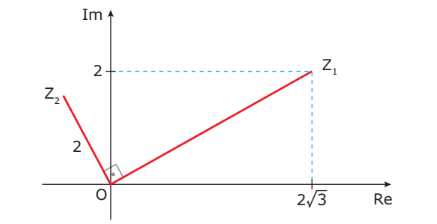
\includegraphics[scale=0.7]{Imagens/L2F1.png}
  \end{figure}

  Se $z_1 \cdot z_2 = a + bi$, então $a + b$ é igual a:
  \begin{enumerate}
    \item $4(1 - \sqrt{3})$
    \item $2(\sqrt{3} - 1)$
    \item $2(1 + \sqrt{3})$
    \item $8(\sqrt{3} - 1)$
    \item $4(\sqrt{3} + 1)$
  \end{enumerate}

  % Questão 03
  \item (UFRGS) O ângulo formado pelas representações geométricas dos números complexos $z = \sqrt{3} + i$ e $z^4$ é:
  \begin{enumerate}
    \item $\dfrac{\pi}{6}$
    \item $\dfrac{\pi}{4}$
    \item $\dfrac{\pi}{3}$
    \item $\dfrac{\pi}{2}$
    \item $\pi$
  \end{enumerate}

  % Questão 05
  \item (UEG) O conjunto dos números complexos que satisfazem a condição $|z - 3i| = |z - 2|$ é representado no plano cartesiano por uma reta:
  \begin{enumerate}
    \item cuja inclinação é positiva.
    \item que contém a origem do sistema.
    \item que não intercepta o eixo real.
    \item cuja inclinação é negativa.
  \end{enumerate}

  % Questão 07
  \item (FUVEST-SP) Entre os números complexos $z = a + bi$, não nulos, que têm argumento igual a $\dfrac{\pi}{4}$, aquele cuja representação geométrica está sobre a parábola $y = x^2$ é:
  \begin{enumerate}
    \item $1 + i$
    \item $1 - i$
    \item $-1 + i$
    \item $\sqrt{2} + 2i$
    \item $-\sqrt{2} + 2i$
  \end{enumerate}

  % Questão 08
  \item (Cesgranrio) O conjunto dos pontos $z = x + yi$ do plano complexo que satisfazem $|z - 1|^2 = 2x$ e $y \ge 2$ é:
  
  \begin{enumerate}
    \item o conjunto vazio.
    \item uma região não limitada do plano.
    \item todos os pontos $x + yi$ tais que $y \ge 2$.
    \item uma reta.
    \item diferente dos quatro anteriores.
  \end{enumerate}

  
  % Questão 16
  \item (UNIFESP) Quatro números complexos representam, no plano complexo, vértices de um paralelogramo. Três dos números são $z_1 = -3 - 3i$, $z_2 = 1$ e $z_3 = -1 + \dfrac{5}{2}i$. O quarto número tem as partes real e imaginária positivas. Esse número é:
  \begin{enumerate}
    \item $2 + 3i$
    \item $3 + \dfrac{11}{2}i$
    \item $3 + 5i$
    \item $2 + \dfrac{11}{2}i$
    \item $4 + 5i$
  \end{enumerate}

  % Questão 10
  \item (UFU-MG) Sejam $z_1$ e $z_2$ dois números complexos representados geometricamente, na figura a seguir, pelos pontos $A$ e $B$ respectivamente.

  \begin{figure}[h!]
    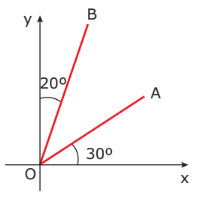
\includegraphics[scale=0.7]{Imagens/L2F3.png}
  \end{figure}

  Sabendo-se que $OA = 3\text{ cm}$ e que $OB = 6\text{ cm}$, pode-se afirmar que:
  \begin{enumerate}
    \item $\dfrac{z_2}{z_1}$ tem módulo igual a $2\text{ cm}$.
    \item $z_1 + z_2$ tem módulo igual a $9\text{ cm}$.
    \item O argumento de $z_2 - z_1$ é igual a $40^\circ$.
    \item O argumento de $z_2 \cdot z_1$ é igual a $50^\circ$.
  \end{enumerate}

\end{enumerate}

%\espacoresposta{4cm}



\end{document}